\section{CAN}

\paragraph{}
Controller Area Network (CAN)\cite{wikipediaCAN} busses are commonly used in automotive applications to connect different control or instrumentation nodes together developed by Bosch in the 1990s.
This allows for any node to communicate with any other node on the bus.
CAN utilizes a two wire asynchronous differential twisted pair signal to transmit across the bus.
The asynchronous nature of this protocol reduces the number of wires required to transmit data.
By utilizing a differential twisted pair, noise and interference are reduced improving reliability and robustness of the network.
However, only utilizing a single differential pair means that a node can only transmit or only receive at any given time, reducing throughput.

\paragraph{}
CAN is an addressed based communication protocol.
An address can correspond to a specific node or to a specific message.
Since CAN only utilizes a single differential signal, it must negotiate to determine which node is transmitting and which nodes are receiving.
The lowest address trying to be transmitted wins the negotiation, meaning that priority can be assigned to messages by assigning a lower value for an address to the message.
This addressing and need to negotiate also adds overhead to the transmission, reducing overall data throughput.
Additionally, there are control bits, cyclical redundancy (CRC) bits, and end of frame (EoF) bits that all also contribute to overhead.

\subsection{CAN 2.0}

\paragraph{}
CAN 2.0\cite{BOSCH_CAN20} is the most commonly used CAN protocol in the automotive.
This version of CAN uses an 11 bit identification or address section with maximum of 8 bytes of data transmitted.
The bitrate for this version of CAN can be up to 1 Mega bit per second (Mbps).
With an assumption of 1 byte of data transmission, the overhead can be computed as $\frac{48 \text{bits}}{56 \text{bits}}$.  With the assumption of 8 bytes of data transmission, the overhead can be computed as $\frac{48 \text{bits}}{112 \text{bits}}$.
The more data that is transmitted per frame, the less overhead impacts the total data throughput.
An example data frame of CAN 2.0 can be seen in \cref{fig:CANDataFrame}.

\begin{figure}[H]
	\centering
	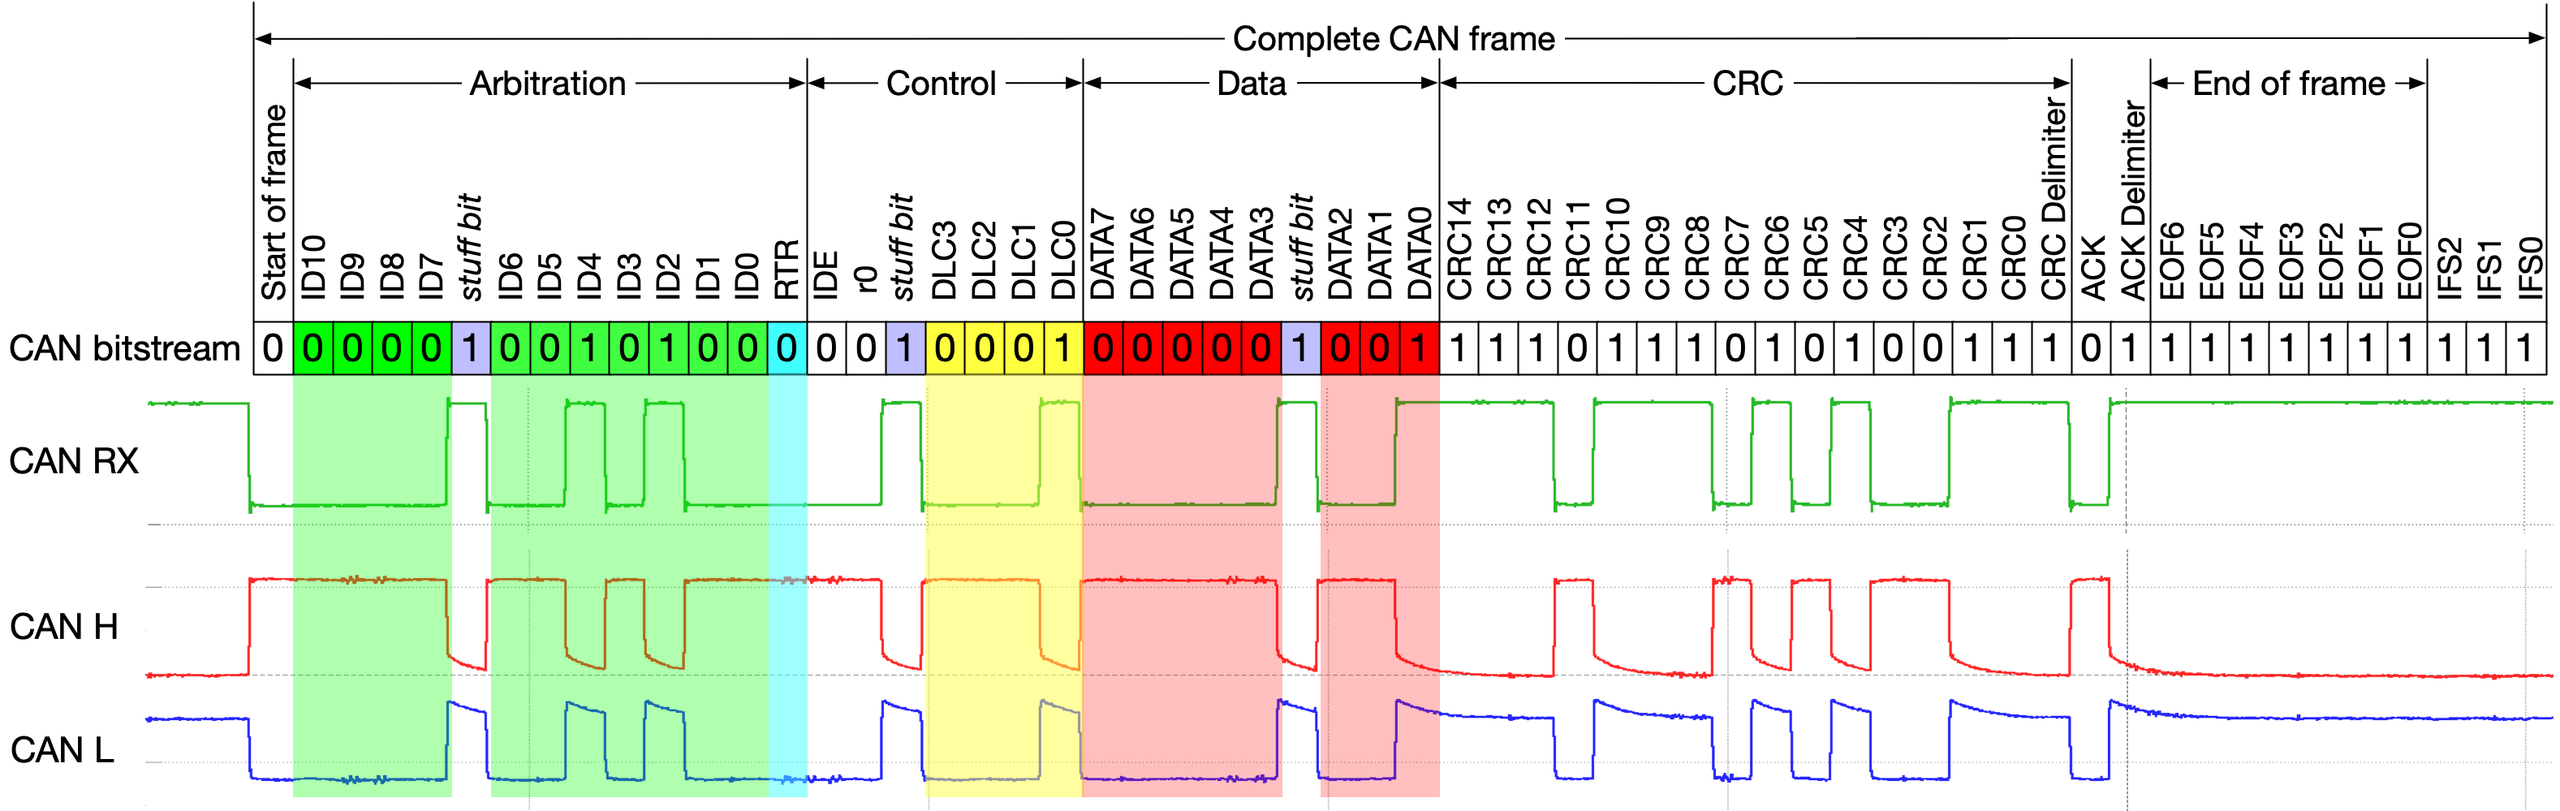
\includegraphics[width=\linewidth]{CAN_20_Frame.png}
	\caption{Example CAN 2.0 Frame \cite{wikipediaCAN}}
	\label{fig:CANDataFrame}
\end{figure}

\subsection{CAN FD}

\paragraph{}
In 2012, Bosch released a new version of CAN with a flexible data rate called CAN FD\cite{BOSCH_CANFD}.
This new version of CAN has several improvements including faster data rates and allowing for more data to be transmitted in each frame.
The flexible data rate comes from CAN FD's ability to increase the data rate during the data section of the transmission.
The protocol supports up to 8 Mbps of throughput during the data section of transmission and up to 1 Mbps of throughput during the beginning and ending parts of the frame.
This allows for significantly more data throughput overall.
In addition to the flexible data rate used by CAN FD, the maximum size of the data section was increased from 8 bytes to 64 bytes.
This decreases total overhead significantly making the transmission more efficient.
These two new characteristics combined provide for a much more efficient transfer of data, particularly when transmitting high amounts of data very frequently.

\paragraph{}
In order to use CAN FD, it must be supported by the hardware, including both the CAN controller and the CAN transceiver.
Additionally, to rely solely on CAN FD, each node on the bus must be using CAN FD.
Otherwise, conflicts may occur impacting frames being sent or received.
The system would theoretically operate without too many issue, but the control section of the frame would be different sizes to accommodate the additional control bits needed for the CAN FD frame.